
\ifnumequal{\value{rolldice}}{0}{
  \renewcommand\va{6}
  \renewcommand\vb{10}
  \renewcommand\vc{6}
  \renewcommand\vx{1}
  \renewcommand\vy{5}
}{
  \ifnumequal{\value{rolldice}}{1}{
    \renewcommand\va{3}
    \renewcommand\vb{8}
    \renewcommand\vc{7}
    \renewcommand\vx{1}
    \renewcommand\vy{4}
  }{
    \ifnumequal{\value{rolldice}}{2}{
      \renewcommand\va{4}
      \renewcommand\vb{12}
      \renewcommand\vc{6}
      \renewcommand\vx{2}
      \renewcommand\vy{3}
    }{
      \renewcommand\va{5}
      \renewcommand\vb{16}
      \renewcommand\vc{7}
      \renewcommand\vx{2}
      \renewcommand\vy{4}
    }
  }
}

\ADD\va\vc\vd 
\DIVIDE\vd{2}\ve
\DIVIDE\vb{2}\vf 

\SQUARE\vy\a
\MULTIPLY\a\vy\b
\MULTIPLY\a\ve\c
\FRACMULT{2}{3}\b{1}\d\e
\MULTIPLY\vb\vy\f

\SQUARE\vx\m
\MULTIPLY\m\vx\n
\MULTIPLY\m\ve\o
\FRACMULT{2}{3}\n{1}\p\q
\MULTIPLY\vb\vx\r

\EXPR[0]\vp{\c-\f-\o+\r}
\FRACMINUS\p\q\d\e\vq\vr
\FRACADD\vp{1}\vq\vr\vm\vn

\question[3] Find the area bounded by the parabolas 
\[ y = x^2-\va x+\vb\text{ and }y=\vc x-x^2 \]
\watchout

\ifprintanswers
  \vspace{0.3cm}
  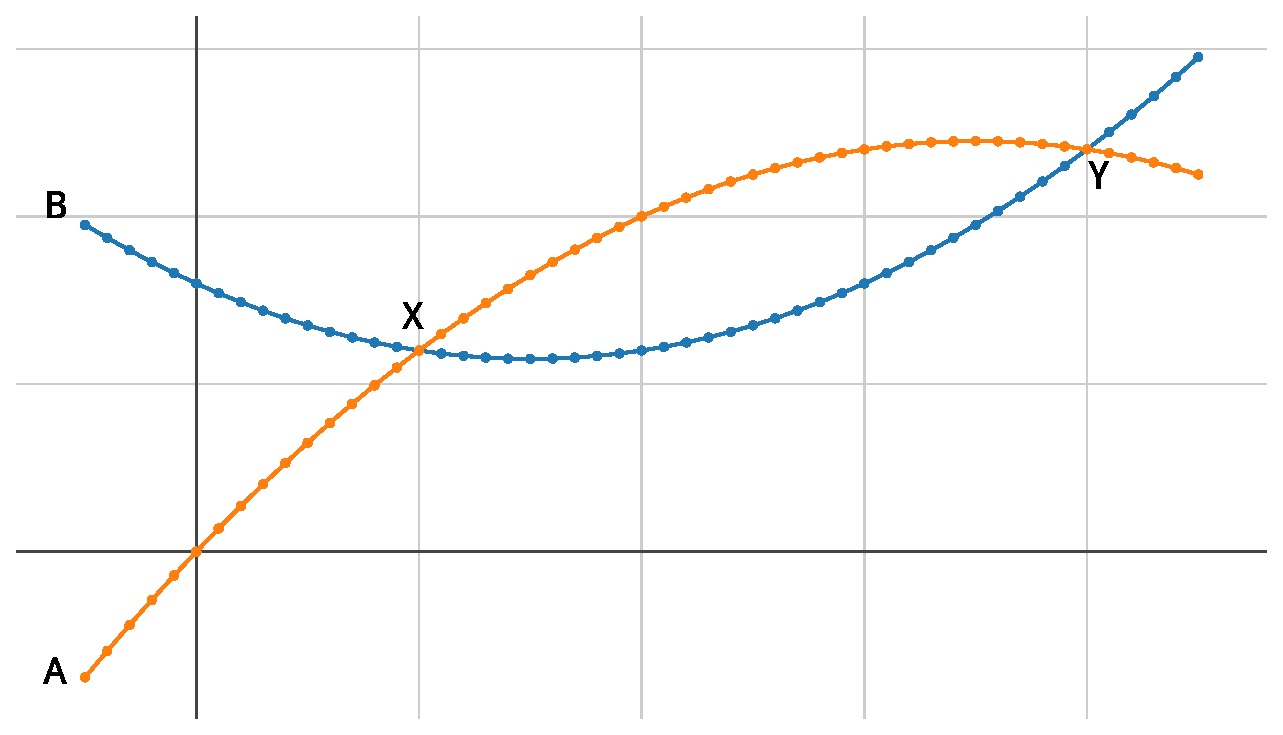
\includegraphics[width=300pt]{plotly.eps}
\fi

\begin{solution}[\fullpage]
	The two parabolas intersect at points ($X$ and $Y$ in the figure) where 
  \begin{align}
    \overbrace{x^2-\va x + \vb}^{B} &= \overbrace{\vc x - x^2}^{A} \\
    \implies 2x^2 - \vd x + \vb &= 0 \\ 
    \implies x^2-\ve x + \vf &= 0 \implies x=\vx,\vy 
  \end{align}
	
	The required area $A$ of region $R$ is therefore
	\begin{align}
	  A &= \int_\vx^\vy\left[ (\vc x-x^2) - (x^2-\va x + \vb)\right]\ud x \\
	    &= \int_\vx^\vy (\vd x - 2x^2 - \vb) \ud x \\
      &= \left[ \ve x^2 -\dfrac{2}{3}x^3 - \vb x\right]_\vx^\vy \\
      &= \left(\c - \dfrac\d\e - \f\right) - \left( \o-\dfrac\p\q - \r\right) = \WRITEFRAC\vm\vn
	\end{align}
\end{solution}

\ifprintanswers\begin{codex}$\WRITEFRAC\vm\vn$\end{codex}\fi
